\documentclass[tikz,border=4pt]{standalone}
\usepackage{amsmath,amssymb}
\usetikzlibrary{arrows.meta}

\begin{document}
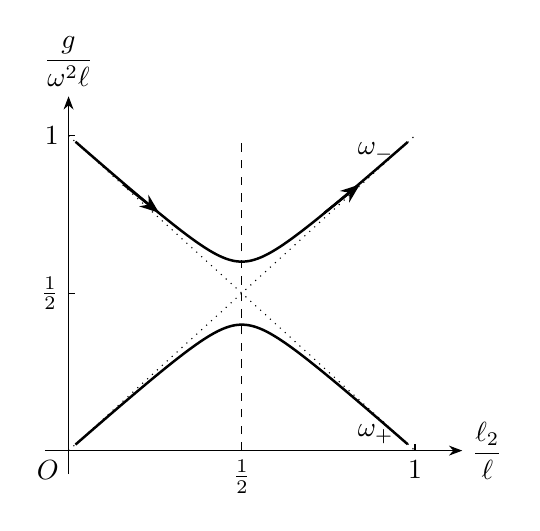
\begin{tikzpicture}[
  >=Stealth,
  font=\normalsize,
  axis/.style={line width=0.4pt},
  curve/.style={line width=0.9pt}
]
  % Axes: x = l_2/l in [0, 1] -> [0, 4.4], y = g/(omega^2 l) in [0, 1] -> [0, 4.0]
  \draw[axis,->] (-0.3,0) -- (5.0,0) node[right] {$\dfrac{\ell_2}{\ell}$};
  \draw[axis,->] (0,-0.3) -- (0,4.5) node[above] {$\dfrac{g}{\omega^2\ell}$};
  \node[below left] at (0,0) {$O$};

  % Ticks 1/2, 1
  \draw[axis] (2.2,0) -- (2.2,0.08);
  \node[below] at (2.2,0) {$\tfrac{1}{2}$};
  \draw[axis] (4.4,0) -- (4.4,0.08);
  \node[below] at (4.4,0) {$1$};
  \draw[axis] (0,2.0) -- (0.08,2.0);
  \node[left] at (0,2.0) {$\tfrac{1}{2}$};
  \draw[axis] (0,4.0) -- (0.08,4.0);
  \node[left] at (0,4.0) {$1$};

  % Uncoupled asymptotes (dotted): y = x and y = 1 - x
  \draw[axis,dotted] (0,0) -- (4.4,4.0);
  \draw[axis,dotted] (0,4.0) -- (4.4,0);
  \draw[axis,dashed] (2.2,0) -- (2.2,4.0);

  % Coupled branches with eps = m_2/(m_1+m_2) = 0.04 (gap = 0.2)
  % y_pm(u) = 0.5*(1 +- sqrt((1-2u)^2 + 4*0.04*u*(1-u)))
  \draw[curve,domain=0.02:0.98,samples=120]
    plot ({4.4*\x}, {4.0*0.5*(1 + sqrt((1-2*\x)^2 + 0.16*\x*(1-\x)))});
  \draw[curve,domain=0.02:0.98,samples=120]
    plot ({4.4*\x}, {4.0*0.5*(1 - sqrt((1-2*\x)^2 + 0.16*\x*(1-\x)))});

  % Adiabatic path arrows along upper branch
  \draw[curve,->] (0.7,3.38) -- (1.15,3.02);
  \draw[curve,->] (3.25,3.02) -- (3.7,3.38);

  % Labels
  \node[above right] at (3.55,3.55) {$\omega_-$};
  \node[below right] at (3.55,0.45) {$\omega_+$};
\end{tikzpicture}
\end{document}
